\section{Baseline Reproduction}

The primary metric for image generation is Fréchet Inception Distance (FID)~\cite{heusel2017fid},
which measures the distributional gap between generated and real images in the feature space of a pretrained
Inception-v3 network. Lower FID indicates better quality and diversity together.

We begin by reproducing the key results of the original REPA paper: faster convergence
in terms of FID and improved stability of model features during training.

\begin{figure}
  \centering
  \begin{subfigure}[b]{0.45\textwidth}
    \centering
    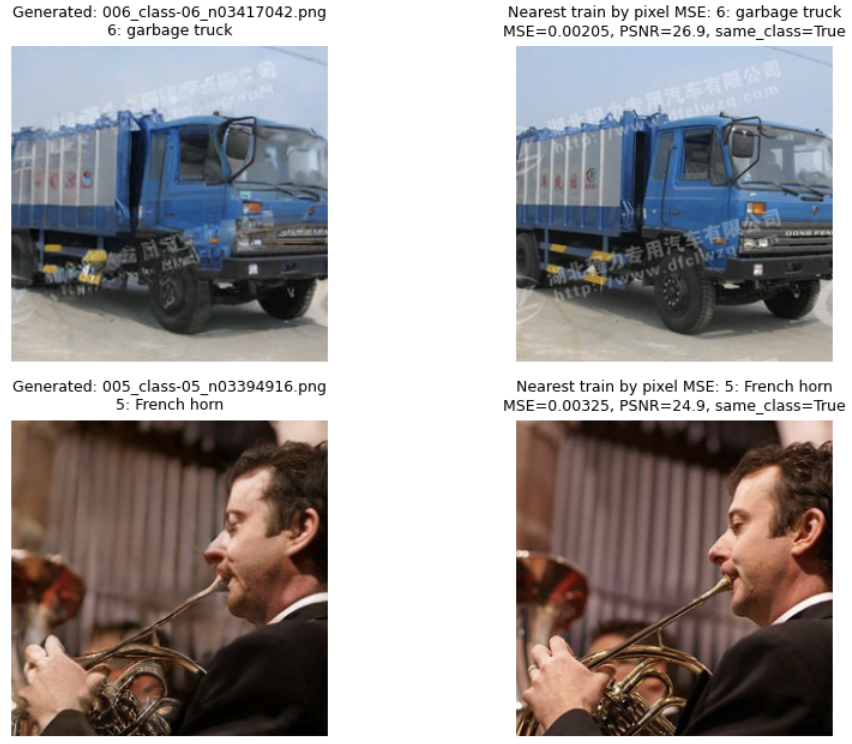
\includegraphics[width=\linewidth]{images/repa_100k_imagenette_mem.png}
    \caption{Imagenette}
    \label{imagenette:memorization}
  \end{subfigure}
  \hfill
  \begin{subfigure}[b]{0.48\textwidth}
    \centering
    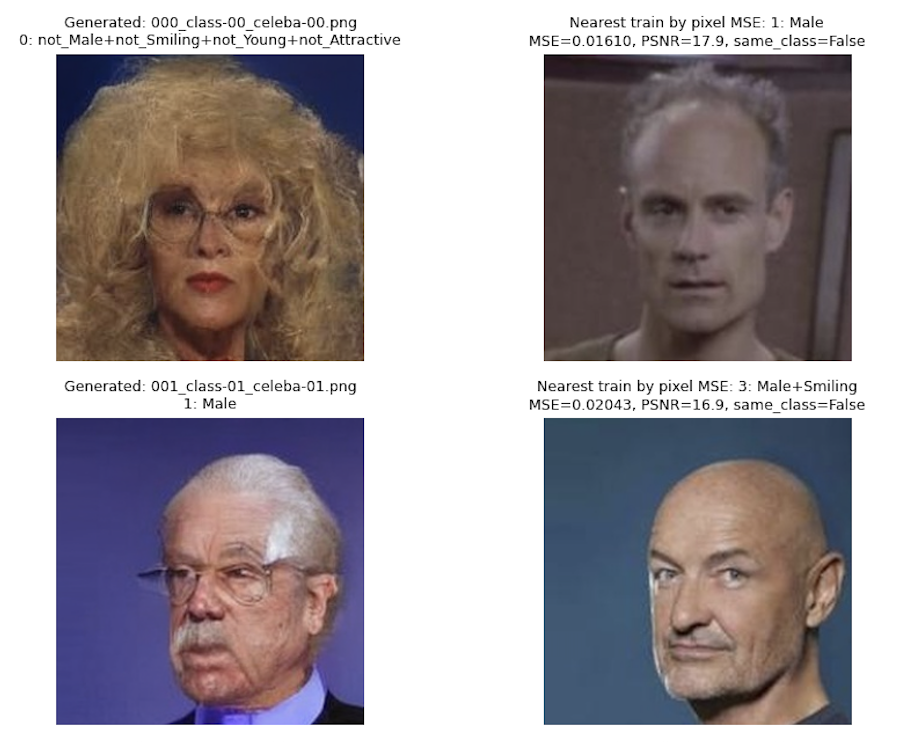
\includegraphics[width=\linewidth]{images/repa_celeba_memorization.png}
    \caption{CelebA}
    \label{celeba:memorization}
  \end{subfigure}
  \caption{Closest dataset images to those generated by diffusion. See full examples in Appendix \ref{app:memorization}.}
  \label{fig:nearest_train_combined}
\end{figure}

\begin{figure}
  \centering
  \begin{subfigure}[b]{0.48\textwidth}
    \centering
    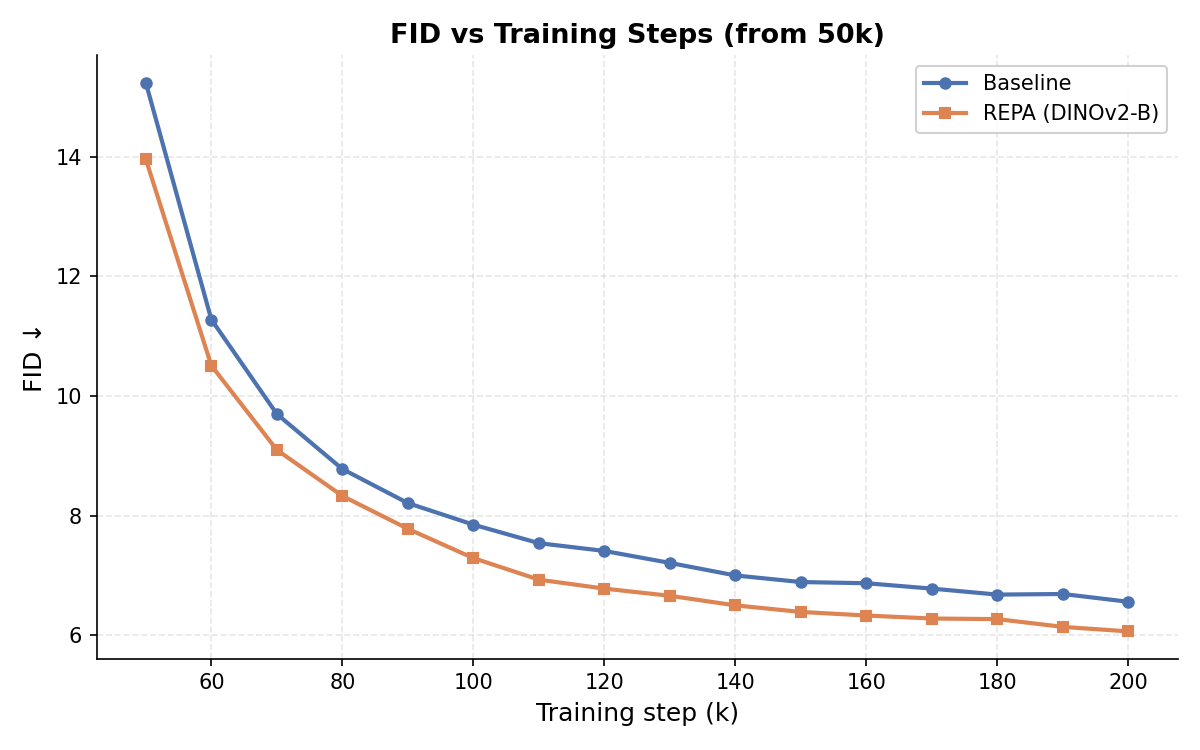
\includegraphics[width=\linewidth]{images/fid_ema.png}
    \caption{FID}
    \label{celeba:fid_ema}
  \end{subfigure}
  \hfill
  \begin{subfigure}[b]{0.48\textwidth}
    \centering
    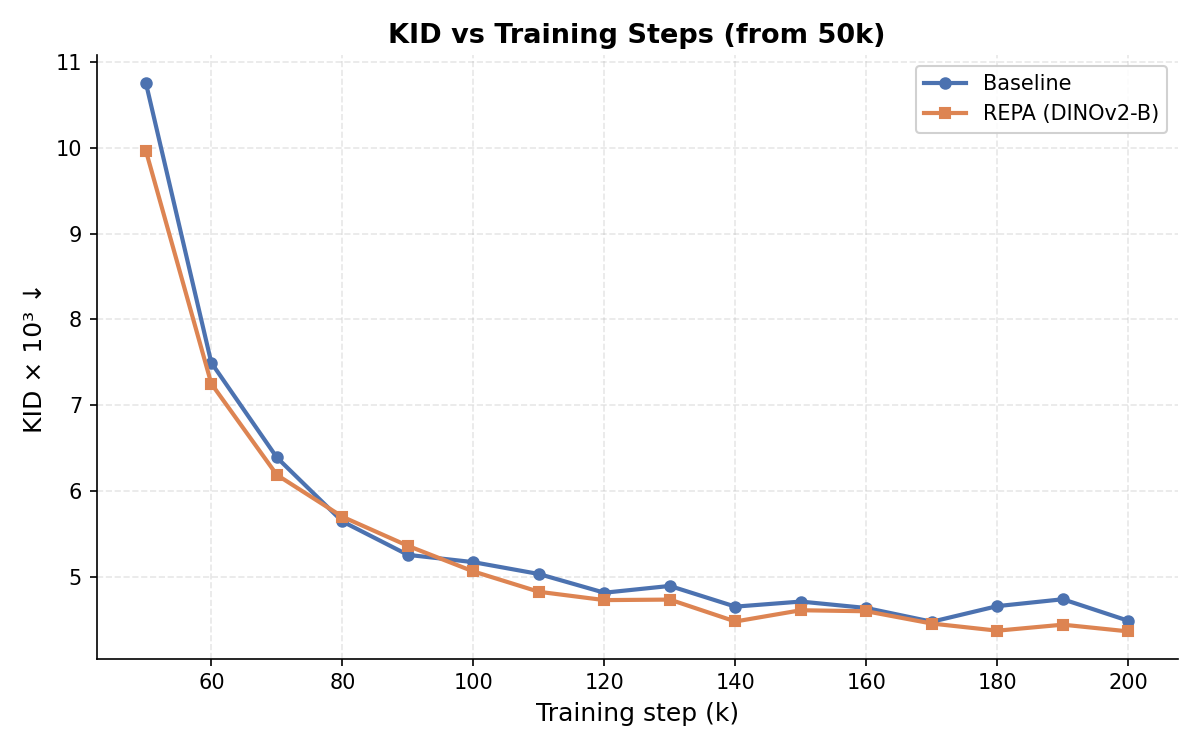
\includegraphics[width=\linewidth]{images/kid_ema.png}
    \caption{KID}
    \label{celeba:kid_ema}
  \end{subfigure}
  \caption{FID and KID plots for training checkpoints}
  \label{fig:memorization_combined}
\end{figure}

\subsection{Imagenette}

We first train on Imagenette -- a subset of ImageNet containing 10 easily classified
classes with approximately 1\,000 samples per class. After 100\,000 iterations the
standard SiT-B/2 model (depth 12, no augmentation) achieves good generation quality,
but at a cost: it is sufficiently large to memorize the entire dataset, a tendency
amplified by the REPA loss, as shown in Figure~\ref{imagenette:memorization}. This
reveals a key risk of applying diffusion models to small-scale datasets -- complete
training set memorization rather than genuine generalization.

\subsubsection{Tackling Memorization}

We mitigate memorization by two complementary strategies. First, we reduce model
capacity: instead of the standard SiT-B/2 (depth 12), we use a shallower variant,
\texttt{SiT-B-shallow/2}, with only 6 transformer blocks while keeping the hidden
dimension (768) and patch size (2) unchanged. Second, we apply random horizontal
flip augmentation to both the raw image and its VAE latent during training. The
corrected model is trained with the DINOv2-vit-s teacher, projection from encoder
depth 4, REPA coefficient $\lambda=0.8$, CFG dropout probability $0.2$, batch size
256, learning rate $10^{-4}$, and gradient clipping at $1.0$ for 100\,000 steps. More
aggressive regularizers (covariance decorrelation, VAE-based random crop) were
explored but did not improve results or destabilized training.

\paragraph{Key Takeaways.} In this section we only present our final results. For
a more detailed discussion about reducing memorization in low-data regimes
we refer the reader to Appendix~\ref{app:memorization}.

The shallow architecture (depth 6) reduces the model's capacity to memorize
the training set while still being expressive enough to learn the target
distribution. The random flip augmentation adds a simple but effective source
of invariance, forcing the model to generalise across horizontally mirrored
views. Together, these changes eliminate memorization on Imagenette.

Even at a lower guidance scale ($w=2.0$), the old model still
shows strong memorization (mean similarity $0.550$, $9\%$ near-copies, accuracy
$51\%$), although the effect is less extreme. This confirms that the problem
is not an artefact of high CFG but a genuine overfitting of the training set.

Our findings have practical implications for REPA in small-data regimes: the
auxiliary alignment loss does not inherently cause memorization, but it can
amplify it when the denoiser is overparameterised. With appropriate capacity
control and basic augmentation, REPA remains a viable training accelerator.
Future work will quantify the convergence speedup on this corrected Imagenette
setup and extend the same anti-memorization protocol to other small-scale
benchmarks.

\subsection{CelebA}
\label{sec:celeba}

Since training on small, multi-domain datasets leads to memorization, we investigate
whether single-domain datasets are subject to this issue as well. We select the
CelebFaces Attributes (CelebA) dataset as our fine-grained benchmark and train the
diffusion model on it. Notably, the memorization problem does not arise here, as
illustrated in Figure~\ref{celeba:memorization}, enabling analysis analogous to that
in the original REPA paper.

\subsubsection{Training Speedup Analysis}

Figure~\ref{fig:memorization_combined} shows FID and KID as a function of training
iteration. Both models improve steadily in generation quality. Contrary to the
trend reported in the original REPA paper, where the alignment term initially
introduced a quality gap, the REPA model begins to benefit from the auxiliary
objective by the first evaluated checkpoint. The improvement is most visible in
FID: at 50\,000 iterations, REPA already improves over the baseline
($\mathrm{FID}\approx 14.0$ versus $\mathrm{FID}\approx 15.2$), and this gap
persists as both models continue to improve, with REPA maintaining lower FID
throughout the evaluated range. Taking the final baseline FID at 200\,000
iterations as a target, REPA reaches comparable quality after roughly
130\,000 -- 140\,000 iterations, corresponding to an approximately $1.5{\times}$
improvement in learning speed. The KID curve supports the same qualitative
conclusion, but less decisively: REPA is also usually below the baseline, yet the
two trajectories are much closer and nearly overlap after the early checkpoints.

After the initial speedup, the two curves become much closer in their rate of
convergence. In both FID and KID, REPA maintains a consistent advantage, but the
gap no longer expands substantially once the models enter the later training
phase. This suggests that REPA primarily accelerates the early formation of useful
representations rather than changing the asymptotic behaviour of the diffusion
objective.

Initially, we hypothesized that after the embedding structure encouraged by the teacher has
already been absorbed, later learning depends increasingly on the standard
diffusion process. To test this hypothesis we track the angle between the two gradients used in
the weight update:

$$
c = \cos(\nabla_{w} \mathcal{L}_{diffusion}, \nabla_{w} \mathcal{L}_{REPA})
$$

Contrary to our assumption, we find that $c$ depends on both noise level and training iteration, varying from highly positive
at high noise levels to negative at lower noise levels and later training iterations (Figure~\ref{fig:grad_compat}, left).
This is in line with the findings presented in~\cite{wang2025haste}. That work suggests simply turning off the extra loss
during later training iterations, but this seems to be too simplistic. Weighting the cosine by the relative gradient
magnitude (the ``useful work'' the alignment term performs, Figure~\ref{fig:grad_compat}, right) shows that the conflict
is concentrated at low noise levels rather than uniformly across training, so we try to develop our own, noise-aware approach.

\begin{figure}
  \centering
  \begin{subfigure}[b]{0.48\textwidth}
    \centering
    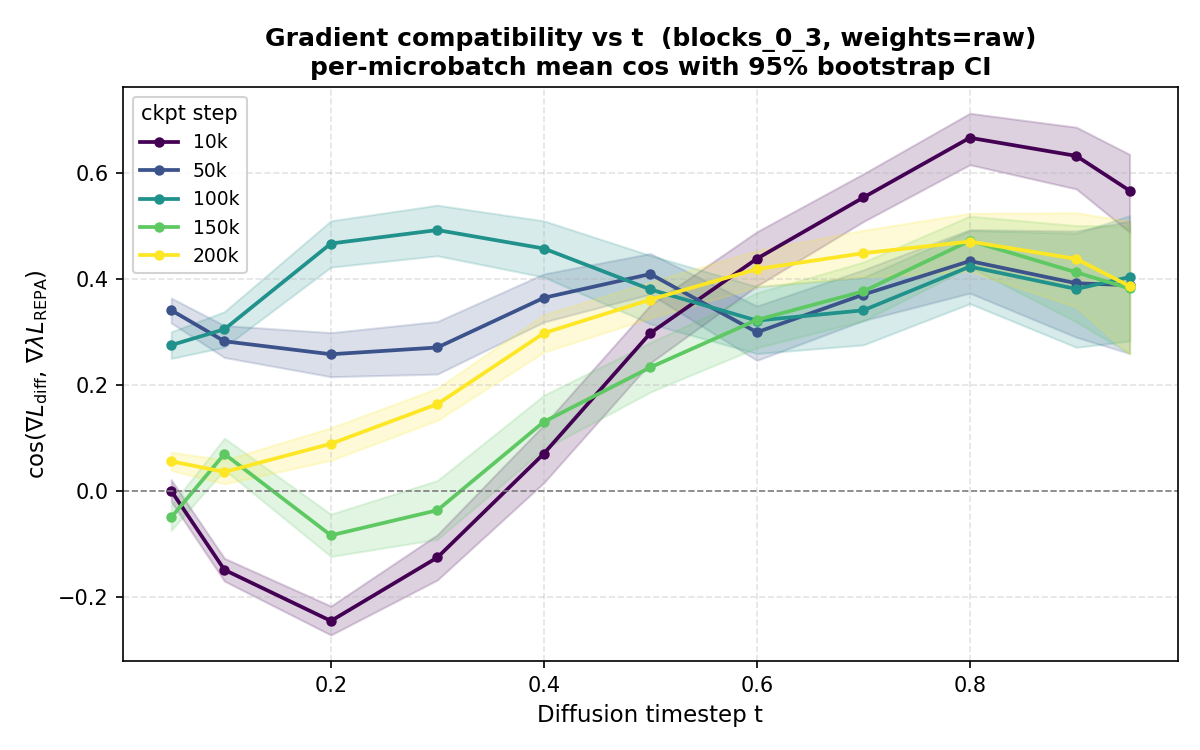
\includegraphics[width=\linewidth]{images/1_cos_vs_t__blocks_0_3__raw.png}
    \caption{Gradient compatibility $c$}
    \label{fig:grad_compat_cos}
  \end{subfigure}
  \hfill
  \begin{subfigure}[b]{0.48\textwidth}
    \centering
    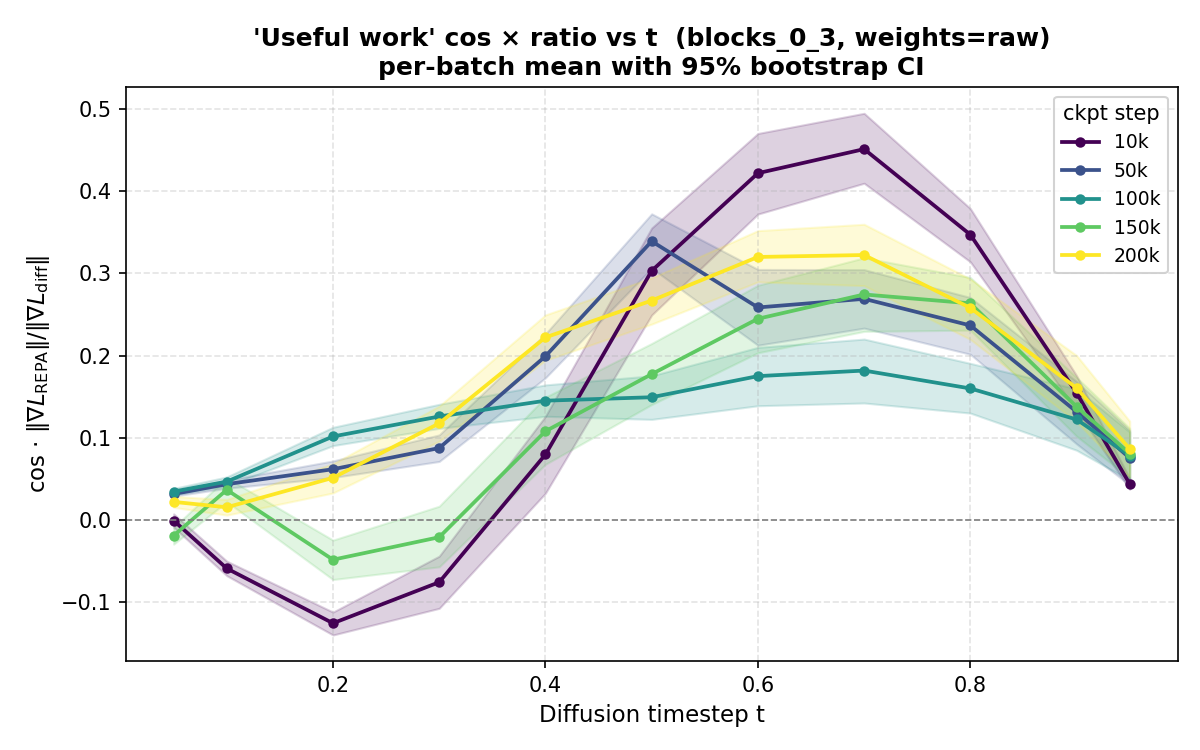
\includegraphics[width=\linewidth]{images/4_useful_work_vs_t__blocks_0_3__raw.png}
    \caption{Useful work ($c \times$ magnitude ratio)}
    \label{fig:grad_compat_work}
  \end{subfigure}
  \caption{Compatibility of the diffusion and REPA gradients in the early transformer blocks (0--3) as a
  function of the diffusion timestep $t$, across training checkpoints. Left: the cosine $c$ is highly positive at high
  noise levels (large $t$) but turns negative at low noise levels and later iterations. Right: weighting $c$ by the
  relative gradient magnitude (``useful work'') localises the conflict to the low-noise regime.}
  \label{fig:grad_compat}
\end{figure}

\subsubsection{Structural Analysis}

To move beyond scalar metrics such as FID and KID, we analyse the internal
representations of both models directly by visualising the patch-level hidden
states at each transformer block. This section describes how those
visualisations are constructed and what they reveal about the effect of REPA
on a face-generation task conditioned on facial attributes.

To do so, we reconstruct PCA feature maps, reproducing the methodology described
in the original REPA paper.

\paragraph{Key Takeaways.} As before, we provide a thorough description of our
experiments and findings in Appendix \ref{app:feature_maps} and only present key takeaways in this section.

CelebA images are spatially homogeneous (face centred, consistent scale), and the
class conditioning is injected at every transformer block via adaptive layer
normalisation, making all 16 class labels trivially linearly decodable from
even the earliest hidden states in both models. The
PCA visualisations serve as the primary evidence for representational
quality, since they reveal the \emph{spatial organisation} of features rather
than their mere linear separability.

The key takeaway is that REPA forces the model to internalise
semantically meaningful facial structure earlier in the network and more
robustly under noise, even though the generation objective alone would not
require it on a spatially homogeneous dataset like CelebA.

As a complementary probe, we analyse whether the trained generator contains
approximately linear directions corresponding to CelebA attributes in its latent
space. The goal is not only to check whether attributes are class-conditionally
decodable, but whether moving along a learned direction produces a controlled
semantic change in generated images.

Both the baseline and REPA models produce coherent
changes as $\alpha$ is varied, indicating that both generators manage
to encode this attribute as an approximately linear vector direction in latent
space.
